\chapter{Populações e demografia}\label{ch:b1:populations}

Um frasco de levedura começa com um milhão de \omterm{def:b1:cell-unit-of-life:cell}{células} e, dezesseis
horas depois, contém sessenta milhões e parou de crescer; uma manada
de veados numa ilha cresce um décimo por ano até o inverno em que o
alimento acaba; os linces da floresta boreal sobem e despencam a cada
dez anos, um ano atrás das lebres que comem. Cada um deles é uma
\emph{\omterm{def:b1:populations:population}{população}} --- os indivíduos de uma espécie num lugar --- e cada
um obedece a uma aritmética que se pode escrever. Este capítulo
descreve como as \omterm{def:b1:populations:population}{populações} são contadas, como seus nascimentos e
mortes são tabulados, as duas equações do crescimento, as forças que
mantêm os números sob controle, e o que a mesma aritmética diz sobre a
nossa própria espécie.

\section{Contar uma população}

\begin{definition}[População, densidade, dispersão]\label{def:b1:populations:population}
\index{população}\index{densidade populacional}
Uma \emph{população} é o conjunto dos indivíduos de uma espécie que
vivem numa dada área num dado momento e podem cruzar entre si. Seu
\emph{tamanho} $N$ é o número de indivíduos; sua \emph{densidade}, o
número por unidade de área ou de volume; sua \emph{dispersão}, o padrão
do espaçamento entre eles --- \emph{agregada} onde os recursos ou a
vida social os reúnem (manadas, cardumes, manchas de uma planta),
\emph{uniforme} onde eles se repelem (aves territoriais, arbustos do
deserto que competem por água), \emph{aleatória} onde nenhum dos dois
atua. As populações têm também uma \emph{estrutura etária}, uma
\emph{razão sexual} e taxas de natalidade, mortalidade, imigração e
emigração, cujo balanço é o crescimento.
\end{definition}

\begin{method}[Estimar uma população]\label{met:b1:populations:counting}
\index{marcação--recaptura}
\begin{enumerate}
  \item \omterm{def:b1:organism-environment:organism}{Organismos} sésseis ou lentos: conte em \emph{quadrados} de
        área conhecida colocados ao acaso, e multiplique a densidade
        média pela área total; a dispersão dos valores entre os
        quadrados dá a precisão e revela o padrão de dispersão.
  \item Animais móveis: \emph{marcação--recaptura}. Capture $M$
        indivíduos, marque-os e solte-os; mais tarde capture $C$, dos
        quais $R$ estão marcados. Se os marcados se misturam
        livremente e nada mudou, a fração de marcados na segunda
        captura é igual à fração de marcados na \omterm{def:b1:populations:population}{população},
        $R/C = M/N$, e portanto $N \approx MC/R$ (a estimativa de
        Lincoln--Petersen).
  \item Verifique as hipóteses: nenhum nascimento, morte ou migração
        entre as capturas, marcas que não caem nem alteram o
        comportamento do animal, capturabilidade igual. Cada falha
        enviesa $N$ num sentido previsível.
  \item Sinais indiretos onde contar é impossível: fezes, pegadas,
        cantos, ninhos, o \omterm{def:b1:nucleic-acids:chain}{DNA} num litro de água de lagoa.
\end{enumerate}
\end{method}

\begin{example}[Ratos-do-campo num prado]\label{ex:b1:populations:voles}
Sessenta ratos-do-campo capturados, marcados e soltos num hectare de
prado; três noites depois oitenta são capturados, dos quais doze trazem
marcas: $N \approx 60\times 80/12 = 400$ ratos, quatro por cem metros
quadrados. Se os ratos marcados, tendo aprendido que as armadilhas
contêm comida, forem capturados com mais facilidade, $R$ fica inflado
e $N$ subestimado; se a marcação os afugentou das armadilhas, o
contrário.
\end{example}

\section{Demografia: nascimentos e mortes por idade}

\begin{definition}[Tabela de vida]\label{def:b1:populations:lifetable}
\index{tabela de vida}\index{sobrevivência}
Uma \emph{tabela de vida} acompanha uma coorte de indivíduos nascidos
juntos ao longo da vida. Para cada idade $x$ ela registra $l_x$, a
\emph{sobrevivência} --- a fração da coorte ainda viva à idade $x$ ---
e $m_x$, a \emph{fecundidade} --- o número médio de filhas nascidas de
uma fêmea de idade $x$. A partir deles: a mortalidade entre idades,
$q_x = 1 - l_{x+1}/l_x$; a \emph{taxa reprodutiva líquida}
$R_0 = \sum_x l_x m_x$, o número de filhas que uma fêmea recém-nascida
terá em média ao longo da vida; e o \emph{tempo de geração}
$T = \sum_x x\,l_x m_x / R_0$, a idade média das mães dessas filhas.
Uma \omterm{def:b1:populations:population}{população} com $R_0 > 1$ cresce, com $R_0 < 1$ decresce; ao longo
de uma geração ela é multiplicada por $R_0$.
\end{definition}

\begin{proposition}[Três formas de curva de sobrevivência]\label{prop:b1:populations:survivorship}
Traçar $\log l_x$ contra a idade dá três tipos de curva. \emph{Tipo
I}: a maioria dos indivíduos sobrevive até a velhice e morre num
intervalo estreito (grandes mamíferos, seres humanos em países ricos).
\emph{Tipo II}: uma probabilidade de morte constante em toda idade,
uma reta em escala logarítmica (muitas aves, lagartos, roedores).
\emph{Tipo III}: mortalidade enorme entre os jovens e vida longa para
os poucos sobreviventes (ostras, peixes, a maioria das plantas e dos
insetos). A forma decorre do modo de vida do \omterm{def:b1:organism-environment:organism}{organismo}: uma espécie
que investe pouco em cada um de muitos descendentes tem uma curva de
tipo III; a que investe muito em cada um de poucos, de tipo I.
\end{proposition}

\begin{omfigure}
\begin{tikzpicture}
\begin{semilogyaxis}[
  width=0.86\linewidth, height=6.2cm,
  axis x line=bottom, axis y line=left,
  xmin=0, xmax=100, ymin=1, ymax=1200,
  xlabel={idade (\% da longevidade máxima)}, ylabel={sobreviventes por 1000 nascidos},
  xlabel style={font=\small, at={(axis description cs:0.5,-0.12)}, anchor=north},
  ylabel style={font=\small},
  tick label style={font=\small}, xtick={0,25,50,75,100}, ytick={1,10,100,1000}, log ticks with fixed point,
  legend style={font=\small, at={(0.03,0.05)}, anchor=south west, draw=none},
  clip=false,
]
\addplot[very thick, omDef, smooth] coordinates {(0,1000) (20,990) (40,970) (60,900) (75,700) (85,400) (92,150) (97,30) (100,1)};
\addlegendentry{tipo I: mamíferos, seres humanos}
\addplot[very thick, omProp, domain=0:100, samples=20] {1000*exp(-0.069*x)};
\addlegendentry{tipo II: aves, roedores}
\addplot[very thick, omThm, smooth] coordinates {(0,1000) (3,100) (10,15) (25,6) (50,4) (75,2.5) (100,1)};
\addlegendentry{tipo III: peixes, ostras, maioria das plantas}
\end{semilogyaxis}
\end{tikzpicture}

{\small Três tipos de curva de \omterm{def:b1:populations:lifetable}{sobrevivência}, em escala logarítmica. O
tipo I morre tarde, o tipo III morre cedo, o tipo II morre a taxa
constante; cada um é uma história de vida escrita como uma linha.}
\end{omfigure}

\begin{omfigure}
\begin{tikzpicture}[font=\footnotesize, line cap=round]
  % two age pyramids: growing (left) and stable (right)
  \foreach \i/\m/\f in {0/4.0/3.8, 1/3.4/3.3, 2/2.8/2.7, 3/2.2/2.2, 4/1.6/1.7, 5/1.1/1.2, 6/0.7/0.8, 7/0.35/0.5} {
    \fill[omDef!55] (-\m,0.5*\i) rectangle (0,0.5*\i+0.42);
    \fill[omThm!45] (0,0.5*\i) rectangle (\f,0.5*\i+0.42);
  }
  \node[anchor=north, align=center] at (0,-0.15) {população em crescimento\\ (muitos jovens)};
  \foreach \i/\m/\f in {0/1.6/1.5, 1/1.7/1.6, 2/1.8/1.7, 3/1.8/1.8, 4/1.7/1.8, 5/1.5/1.7, 6/1.1/1.4, 7/0.6/0.9} {
    \fill[omDef!55] (8.8-\m,0.5*\i) rectangle (8.8,0.5*\i+0.42);
    \fill[omThm!45] (8.8,0.5*\i) rectangle (8.8+\f,0.5*\i+0.42);
  }
  \node[anchor=north, align=center] at (8.8,-0.15) {população estável ou envelhecida\\ (classes etárias uniformes)};
  \foreach \i/\l in {0/0--9, 2/20--29, 4/40--49, 6/60--69} { \node[anchor=east, font=\scriptsize] at (-4.3,0.5*\i+0.21) {\l}; }
  \node[anchor=south, omDef!70!black] at (-2.0,4.1) {machos}; \node[anchor=south, omThm!80!black] at (2.0,4.1) {fêmeas};
\end{tikzpicture}

{\small Pirâmides etárias: o número de indivíduos em cada classe de
idade, machos à esquerda, fêmeas à direita. Uma base larga significa
muitos jovens e crescimento por vir; classes uniformes significam
reposição; uma base estreita significa declínio.}
\end{omfigure}

\begin{example}[Uma tabela de vida para uma manada de veados]\label{ex:b1:populations:deer}
De mil filhotes, seiscentos chegam ao primeiro aniversário, e os
sobreviventes perdem então um décimo do seu número a cada ano até que
poucos passem dos nove; as fêmeas parem a partir dos dois anos, cerca
de oito décimos de uma filha por ano no auge. Somar $l_x m_x$ dá
$R_0 \approx 1.5$: cada fêmea deixa uma filha e meia, e a manada cresce
metade a cada geração de cerca de quatro anos --- um aumento de onze
por cento ao ano até que algo a detenha.
\end{example}

\section{O crescimento}

\begin{theorem}[Crescimento exponencial]\label{thm:b1:populations:exponential}
\index{crescimento exponencial}\index{taxa intrínseca de crescimento}
Uma \omterm{def:b1:populations:population}{população} cujas taxas per capita de natalidade e de mortalidade
$b$ e $d$ são constantes cresce a uma taxa proporcional ao seu tamanho,
\[
\frac{\dd N}{\dd t} = rN, \qquad r = b - d, \qquad N(t) = N_0\,e^{rt},
\]
onde $r$ é a \emph{\omterm{thm:b1:populations:exponential}{taxa intrínseca de crescimento}}. Ela duplica a cada
$\ln 2/r$; uma \omterm{def:b1:populations:population}{população} com $r = \qty{0.11}{yr^{-1}}$ duplica em
\qty{6.3}{yr}, uma com $r = \qty{0.5}{h^{-1}}$ em \qty{83}{min}. A
partir de uma \omterm{def:b1:populations:lifetable}{tabela de vida}, $r \approx \ln R_0 / T$.
\end{theorem}
\begin{proof}
Num intervalo curto $\dd t$ os nascimentos são $bN\,\dd t$ e as mortes
$dN\,\dd t$, de modo que $\dd N = (b - d)N\,\dd t$; a equação
$\dd N/\dd t = rN$ tem por solução $N_0 e^{rt}$ (a derivada de
$e^{rt}$ é $re^{rt}$). Duplicação: $e^{rt} = 2$ dá $t = \ln 2/r$. Ao
longo de uma geração $T$ a \omterm{def:b1:populations:population}{população} é multiplicada por
$R_0 = e^{rT}$, donde $r = \ln R_0/T$.
\end{proof}

\begin{theorem}[Crescimento logístico]\label{thm:b1:populations:logistic}
\index{crescimento logístico}\index{capacidade de suporte}
Se a taxa de crescimento per capita cai linearmente à medida que a
\omterm{def:b1:populations:population}{população} se aproxima de uma \emph{\omterm{thm:b1:populations:logistic}{capacidade de suporte}} $K$ --- o
tamanho que o ambiente consegue sustentar ---
\[
\frac{\dd N}{\dd t} = rN\left(1 - \frac{N}{K}\right), \qquad
N(t) = \frac{K}{1 + \dfrac{K - N_0}{N_0}\,e^{-rt}} .
\]
O crescimento é quase exponencial enquanto $N \ll K$, é máximo em
$N = K/2$ (onde $\dd N/\dd t = rK/4$) e anula-se em $N = K$, valor de
que a \omterm{def:b1:populations:population}{população} se aproxima como de um patamar: uma curva em S.
\end{theorem}
\begin{proof}
Escreva a equação como $\dd N/[N(1 - N/K)] = r\,\dd t$ e separe o lado
esquerdo em $\dd N/N + \dd N/(K - N)$; integrando obtém-se
$\ln[N/(K - N)] = rt + \text{const}$, e resolver para $N$ com $N(0) =
N_0$ dá a fórmula. Derivar $rN(1 - N/K)$ em relação a $N$ e igualar a
zero dá o máximo em $N = K/2$.
\end{proof}

\begin{omfigure}
\begin{tikzpicture}
\begin{axis}[
  width=0.86\linewidth, height=6.4cm,
  axis x line=bottom, axis y line=left,
  xmin=0, xmax=18, ymin=0, ymax=800,
  xlabel={tempo (h)}, ylabel={células de levedura por mL ($\times 10^5$)},
  xlabel style={font=\small, at={(axis description cs:0.5,-0.12)}, anchor=north},
  ylabel style={font=\small},
  tick label style={font=\small}, xtick={0,4,8,12,16}, ytick={0,200,400,600,800},
  legend style={font=\small, at={(0.03,0.97)}, anchor=north west, draw=none},
  clip=false,
]
\addplot[very thick, omDef, domain=0:18, samples=100] {660/(1+65*exp(-0.53*x))};
\addlegendentry{logística, $K = 660$, $r = \qty{0.53}{h^{-1}}$}
\addplot[thick, dashed, omThm, domain=0:9, samples=50, restrict y to domain=0:800] {10*exp(0.53*x)};
\addlegendentry{exponencial com o mesmo $r$}
\addplot[only marks, mark=*, mark size=1.8pt, omDef!70!black] coordinates {(0,10) (2,29) (4,71) (6,175) (8,351) (10,513) (12,595) (14,641) (16,656)};
\draw[dashed, gray] (axis cs:0,660) -- (axis cs:18,660); \node[font=\scriptsize, anchor=south east] at (axis cs:18,662) {$K$};
\draw[dashed, gray] (axis cs:0,330) -- (axis cs:7.9,330); \node[font=\scriptsize, anchor=west] at (axis cs:8.2,300) {crescimento mais rápido em $K/2$};
\end{axis}
\end{tikzpicture}

{\small Uma cultura de levedura contada de duas em duas horas
(pontos), a curva logística ajustada a ela, e a exponencial que ela
teria seguido sem limite. As duas concordam nas primeiras seis horas e
depois se separam.}
\end{omfigure}

\begin{proposition}[Dependência da densidade]\label{prop:b1:populations:densitydependence}
\index{dependência da densidade}
O crescimento desacelera à medida que a densidade sobe porque a taxa
de natalidade per capita cai ou a de mortalidade sobe com a
aglomeração: o alimento por cabeça diminui, os territórios ficam
indisponíveis, os dejetos e as doenças se acumulam, os predadores se
concentram. Esses fatores \emph{dependentes da densidade} regulam a
\omterm{def:b1:populations:population}{população} rumo a $K$. Os fatores \emph{independentes da densidade} ---
geada, enchente, fogo, seca --- matam uma fração seja qual for o
número e não podem regular, apenas perturbar; as \omterm{def:b1:populations:population}{populações} de muitos
insetos são governadas sobretudo pelo tempo atmosférico e nunca se
aproximam de uma \omterm{thm:b1:populations:logistic}{capacidade de suporte}.
\end{proposition}
\begin{proof}[Evidências]
Gause (1934) cultivou \emph{Paramecium} em tubos de meio renovado
diariamente: as contagens seguiram uma curva logística até um patamar
fixado pelo alimento, e duplicar o alimento duplicou o patamar. Pearl
(1927) encontrou o mesmo em moscas-das-frutas em frascos, e Carlson
(1913) em levedura. No campo, os pardais-cantores de uma ilha põem
ninhadas menores e perdem mais filhotes quando a \omterm{def:b1:populations:population}{população} reprodutora
é grande, e o número de territórios limita o número de reprodutores;
retirar aves é seguido pela sua reposição a partir de um excedente que
estivera excluído.
\end{proof}

\begin{definition}[Estratégias de história de vida]\label{def:b1:populations:rK}
\index{estratégia r}\index{estratégia K}
As espécies diferem quanto ao lugar que ocupam entre dois extremos.
Uma espécie \emph{$r$-selecionada} --- ervas daninhas, pulgões,
camundongos, a maioria dos peixes --- é feita para um $r$ alto:
amadurece cedo, produz muitos descendentes pequenos, investe pouco em
cada um, vive pouco e explora hábitats novos ou perturbados antes que
a concorrência chegue, com \omterm{def:b1:populations:lifetable}{sobrevivência} de tipo III. Uma espécie
\emph{$K$-selecionada} --- carvalhos, elefantes, albatrozes --- é feita
para persistir perto de $K$: amadurece tarde, produz poucos
descendentes grandes, cuida deles, vive muito, compete bem em hábitats
estáveis e povoados, com uma curva de tipo I. A maioria das espécies
mistura as duas coisas; os rótulos nomeiam as pontas da escala.
\end{definition}

\section{Flutuação e regulação}

\begin{proposition}[Ciclos de predador e presa]\label{prop:b1:populations:cycles}
\index{ciclo populacional}
Algumas \omterm{def:b1:populations:population}{populações} não se estabilizam: oscilam. A lebre-americana da
floresta setentrional e o lince que a come sobem e descem juntos com
um período de cerca de dez anos, o lince um ano ou dois atrás da
lebre: muitas lebres alimentam muitos linces, muitos linces reduzem as
lebres, poucas lebres fazem os linces passar fome, poucos linces
deixam as lebres recuperar-se. O ciclo é impelido em parte pelo
predador e em parte pelo próprio alimento das lebres, cuja recuperação
depois do excesso de pastejo leva anos; modelos de predador e presa
acoplados (\cref{ch:b1:species-interactions}) reproduzem tais
oscilações a partir de duas equações.
\end{proposition}
\begin{proof}[Evidências]
Os registros de peles de uma companhia comercial, mantidos por noventa
anos a partir da década de 1840, anotam o número de peles de lince e
de lebre entregues a cada ano em todo um subcontinente: as duas séries
mostram picos a cada nove ou dez anos, com o pico do lince atrasado em
relação ao da lebre, ao longo de nove ciclos completos. Estudos de
campo posteriores, com lebres cercadas contra predadores ou com
alimento extra, mostram que remover qualquer um dos fatores amortece o
ciclo e remover os dois o abole.
\end{proof}

\begin{omfigure}
\begin{tikzpicture}
\begin{axis}[
  width=0.9\linewidth, height=6.0cm,
  axis x line=bottom, axis y line=left,
  xmin=1845, xmax=1935, ymin=0, ymax=160,
  xlabel={ano}, ylabel={peles comercializadas (milhares)},
  xlabel style={font=\small, at={(axis description cs:0.5,-0.12)}, anchor=north},
  ylabel style={font=\small},
  tick label style={font=\small, /pgf/number format/1000 sep=}, xtick={1850,1870,1890,1910,1930}, ytick={0,50,100,150},
  legend style={font=\small, at={(0.97,0.97)}, anchor=north east, draw=none},
  clip=false,
]
\addplot[very thick, omProp, smooth] coordinates {(1845,20) (1848,50) (1851,120) (1853,40) (1856,15) (1859,60) (1862,140) (1864,60) (1867,20) (1870,50) (1873,100) (1876,30) (1879,12) (1882,70) (1885,150) (1888,40) (1891,20) (1894,50) (1897,100) (1900,30) (1903,15) (1906,60) (1909,120) (1912,30) (1915,15) (1918,50) (1921,110) (1924,40) (1927,15) (1930,60) (1933,100)};
\addlegendentry{lebre-americana}
\addplot[very thick, omDef, smooth] coordinates {(1845,10) (1849,20) (1852,45) (1855,20) (1858,8) (1861,25) (1864,60) (1866,25) (1869,10) (1872,30) (1875,40) (1878,15) (1881,10) (1884,40) (1887,70) (1890,20) (1893,10) (1896,30) (1899,45) (1902,15) (1905,8) (1908,35) (1911,55) (1914,15) (1917,8) (1920,30) (1923,50) (1926,15) (1929,10) (1932,30) (1935,45)};
\addlegendentry{lince}
\end{axis}
\end{tikzpicture}

{\small Peles de lebre e de lince levadas aos postos comerciais da
floresta setentrional, ano a ano (suavizadas). As duas ciclam com um
período de cerca de dez anos, o lince um ano ou dois atrás da lebre.}
\end{omfigure}

\begin{omfigure}
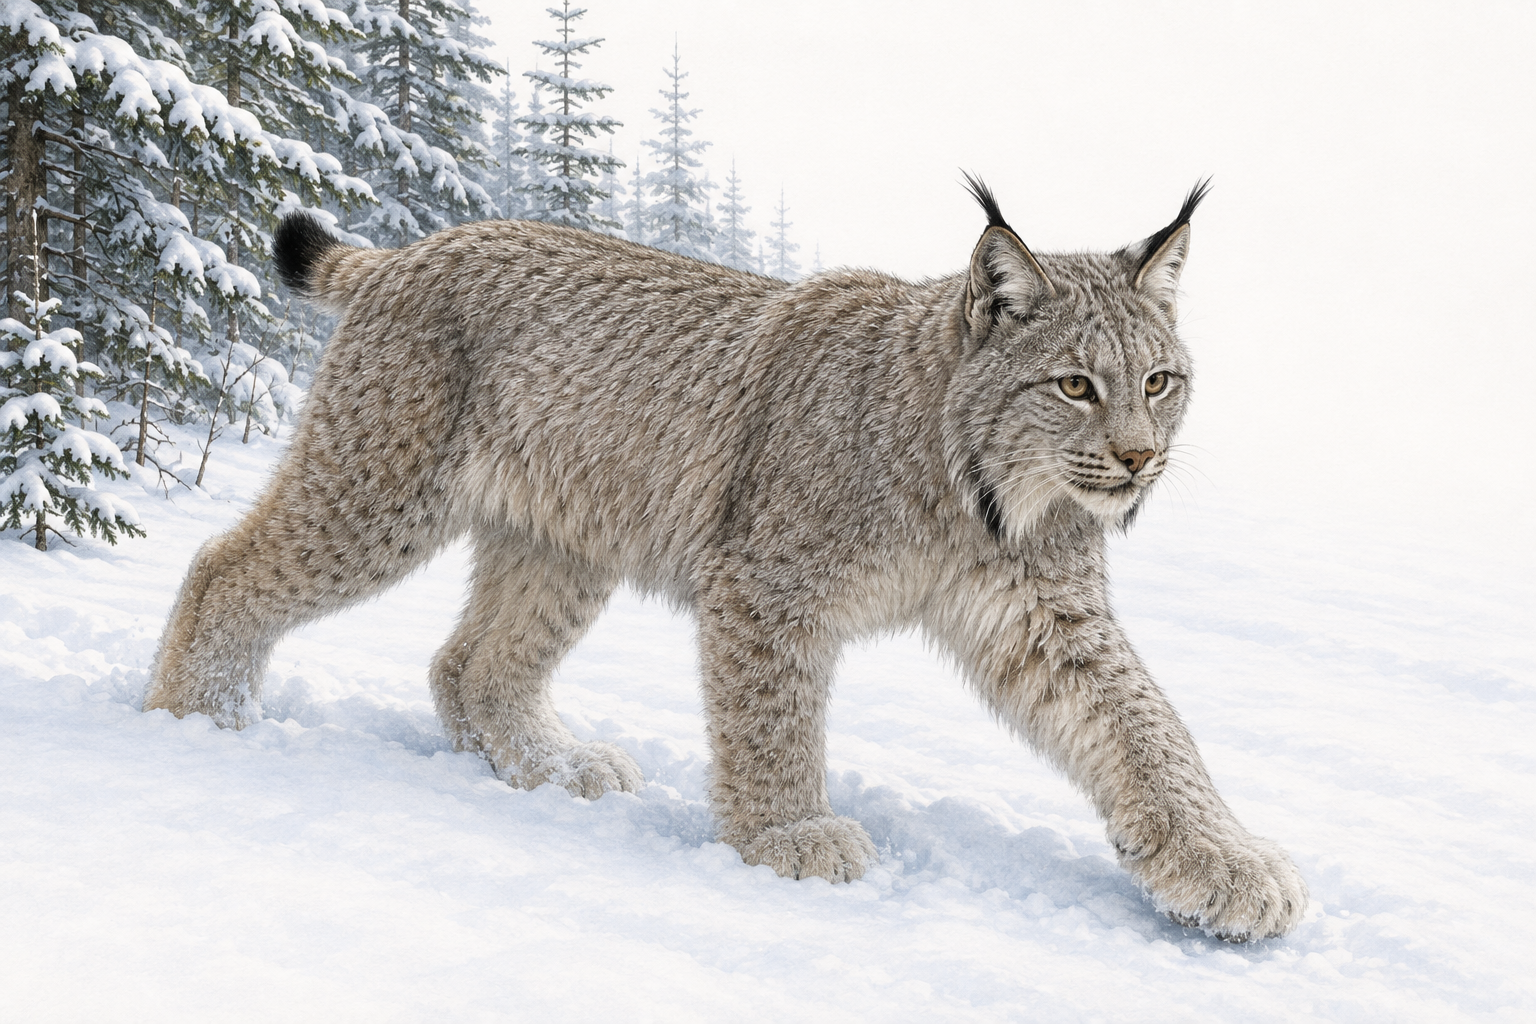
\includegraphics[width=0.52\linewidth]{images/book3/ai/b3-25-lynx-snow.png}

{\small Um lince na floresta boreal. Seus números seguem os da lebre
com um atraso: o ciclo do predador é o da presa, retardado.}
\end{omfigure}

\begin{example}[A nossa própria espécie]\label{ex:b1:populations:humans}
A \omterm{def:b1:populations:population}{população} humana levou toda a história para chegar a um bilhão, por
volta de 1800, e dois séculos para chegar a oito. Sua taxa de
crescimento atingiu o pico perto de \qty{2}{\%} ao ano na década de
1960 (duplicação em 35 anos) e desde então caiu abaixo de
\qty{1}{\%}, não pelas mortes mas pelos nascimentos: onde a
mortalidade infantil cai e as mulheres são educadas, as famílias
encolhem em uma geração, e a pirâmide etária passa de triângulo a
coluna. A aritmética de $R_0$ vale para nós; o que mudou foi $m_x$.
\end{example}

\section{Exercícios}

\begin{exercise}[$\star$]\label{exo:b1:populations:1}
Defina \omterm{def:b1:populations:population}{população}, densidade e dispersão, e dê um exemplo de cada
padrão de dispersão.
\end{exercise}

\begin{exercise}[$\star$]\label{exo:b1:populations:2}
Defina $l_x$, $m_x$, $R_0$ e $T$, e diga o que significa $R_0 = 1$.
\end{exercise}

\begin{exercise}[$\star$]\label{exo:b1:populations:3}
A partir da figura das curvas de \omterm{def:b1:populations:lifetable}{sobrevivência}, que fração de uma
coorte de tipo III sobrevive ao primeiro décimo da sua longevidade? E
de uma coorte de tipo I, que fração chega a três quartos dela?
\end{exercise}

\begin{exercise}[$\star$]\label{exo:b1:populations:4}
Enuncie as equações exponencial e logística e diga o que significam
$r$ e $K$.
\end{exercise}

\begin{exercise}[$\star\star$]\label{exo:b1:populations:5}
Uma cultura de bactérias cresce de $10^4$ a $10^7$ \omterm{def:b1:cell-unit-of-life:cell}{células} por
mililitro em \qty{5}{h}. Calcule $r$ e o tempo de duplicação.
\end{exercise}

\begin{exercise}[$\star\star$]\label{exo:b1:populations:6}
Uma \omterm{def:b1:populations:lifetable}{tabela de vida}: $l_x = 1, 0.5, 0.3, 0.1, 0$ nas idades 0 a 4; $m_x = 0,
1, 2, 2, 0$. Calcule $R_0$, $T$ e $r$, e diga se a \omterm{def:b1:populations:population}{população} cresce.
\end{exercise}

\begin{exercise}[$\star\star$]\label{exo:b1:populations:7}
Cinquenta peixes são marcados e soltos num lago; uma semana depois 70
são capturados, 7 marcados. Estime $N$. Se dez dos peixes marcados
morreram por causa do manuseio, a estimativa fica alta ou baixa demais,
e por quanto?
\end{exercise}

\begin{exercise}[$\star\star$]\label{exo:b1:populations:8}
Uma \omterm{def:b1:populations:population}{população} logística tem $K = 1000$ e $r = \qty{0.2}{yr^{-1}}$.
Calcule $\dd N/\dd t$ em $N = 100$, $500$ e $900$, e o número máximo
que pode ser colhido a cada ano sem declínio.
\end{exercise}

\begin{exercise}[$\star\star$]\label{exo:b1:populations:9}
Classifique como $r$- ou $K$-selecionadas, com dois traços cada: um
dente-de-leão, um elefante, um bacalhau, um gorila, uma mosca-doméstica.
\end{exercise}

\begin{exercise}[$\star\star\star$]\label{exo:b1:populations:10}
A partir da figura da levedura, estime $r$ pelos dois primeiros pontos
e $K$ pelos últimos, depois preveja $N$ a \qty{8}{h} pela fórmula
logística e compare com a contagem. Em que instante a taxa de
crescimento é máxima, e quanto vale?
\end{exercise}

\begin{exercise}[$\star\star\star$]\label{exo:b1:populations:11}
Explique por que um fator independente da densidade não pode regular
uma \omterm{def:b1:populations:population}{população} embora possa reduzi-la, usando as equações, e por que as
\omterm{def:b1:populations:population}{populações} de insetos governadas pelo tempo atmosférico mesmo assim
não crescem sem limite.
\end{exercise}

\begin{exercise}[$\star\star\star$]\label{exo:b1:populations:12}
``Uma \omterm{def:b1:populations:population}{população} não é um número, mas uma distribuição.'' Discuta num
parágrafo: a estrutura etária, o atraso entre uma queda de $m_x$ e uma
queda de $N$, e o que uma pirâmide prevê que $N$ sozinho não prevê.
\end{exercise}

\section{Problema: Levedura num frasco e veados numa ilha}

\begin{problem}[{Problema de fim de semana --- uma cultura contada, uma
manada tabulada, um lago amostrado e uma colheita fixada, terminando na
capacidade de suporte e na taxa intrínseca de crescimento da levedura}]
\label{pb:b1:populations:1}
Uma cultura de levedura é contada de duas em duas horas (\omterm{def:b1:cell-unit-of-life:cell}{células} por
mililitro, $\times 10^5$): $10, 29, 71, 175, 351, 513, 595, 641, 656$ em $t = 0,
2, \ldots, 16$ h. Uma \omterm{def:b1:populations:population}{população} de veados numa ilha tem a \omterm{def:b1:populations:lifetable}{tabela de
vida}: $l_x = 1.00, 0.60, 0.52, 0.46, 0.40, 0.34, 0.26, 0.16, 0.06, 0$ e
$m_x = 0, 0, 0.6, 0.8, 0.8, 0.8, 0.7, 0.5, 0.3, 0$ para $x = 0$ a $9$
anos. Num lago, 120 percas são marcadas e soltas; uma semana depois
150 são capturadas, 18 marcadas.

\medskip
\noindent\textbf{Parte I --- A levedura.}
\begin{enumerate}
  \item Estime $r$ pelas duas primeiras contagens, supondo \omterm{thm:b1:populations:exponential}{crescimento
        exponencial} nas duas primeiras horas.
  \item Calcule o tempo de duplicação.
  \item Estime $K$ pelas últimas contagens.
  \item Calcule a previsão logística em $t = 4$, $8$ e \qty{12}{h} e
        compare com as contagens.
  \item Em que \omterm{def:b1:populations:population}{população} o crescimento é mais rápido, e quando ela é
        atingida? Calcule a taxa máxima de crescimento em \omterm{def:b1:cell-unit-of-life:cell}{células} por
        mililitro por hora.
  \item O que o modelo exponencial preveria a \qty{12}{h}? Por que
        fator ele erra?
  \item Nomeie duas coisas que poderiam fixar $K$ num frasco fechado
        de levedura.
\end{enumerate}

\medskip
\noindent\textbf{Parte II --- Os veados.}
\begin{enumerate}[resume]
  \item Calcule a mortalidade $q_x$ no primeiro ano e no quinto. De
        que tipo de \omterm{def:b1:populations:lifetable}{sobrevivência} se trata?
  \item Calcule $l_x m_x$ para cada idade e some: $R_0$.
  \item Calcule $T$.
  \item Calcule $r$ e o tempo de duplicação da manada.
  \item A ilha tem hoje 200 veados. Preveja o número em 10 anos por
        \omterm{thm:b1:populations:exponential}{crescimento exponencial}.
  \item A ilha consegue alimentar 600 veados. Preveja o número em 10
        anos por \omterm{thm:b1:populations:logistic}{crescimento logístico}, e o ano em que a manada passa
        de 500.
\end{enumerate}

\medskip
\noindent\textbf{Parte III --- As percas e a colheita.}
\begin{enumerate}[resume]
  \item Estime a \omterm{def:b1:populations:population}{população} de percas do lago.
  \item Se 20 das percas marcadas perderam suas marcas antes da
        segunda captura, refaça o cálculo com o número verdadeiro de
        peixes marcados, e indique o sentido do erro da primeira
        estimativa.
  \item A \omterm{def:b1:populations:population}{população} de percas tem $K = 1000$ e $r = \qty{0.4}{yr^{-1}}$.
        Calcule a produção máxima sustentável e a \omterm{def:b1:populations:population}{população} em que ela
        é obtida.
  \item Calcule o tempo de duplicação da \omterm{def:b1:populations:population}{população} de percas quando
        ela está muito abaixo de $K$.
  \item O clube decide, em vez disso, retirar \qty{20}{\%} fixos do
        estoque a cada ano. Calcule a \omterm{def:b1:populations:population}{população} de equilíbrio e a
        captura anual nesse equilíbrio.
  \item Um clube de pescadores retira 120 percas por ano. Mostre se a
        \omterm{def:b1:populations:population}{população} consegue sustentá-lo, calculando $\dd N/\dd t$ em $N =
        500$ e em $N = 300$.
  \item Por que colher em $K/2$ é arriscado na prática, tendo em mente
        o tempo atmosférico e o erro de contagem da questão 14?
\end{enumerate}

\medskip
\noindent\textbf{Parte IV --- A regulação.}
\begin{enumerate}[resume]
  \item O $m_x$ dos veados cai à metade quando a manada ultrapassa
        400. Mostre que $R_0$ cai então abaixo de 1 --- o que isso faz
        à manada, e que tipo de fator está em ação?
  \item Um inverno rigoroso mata \qty{40}{\%} dos veados
        independentemente do seu número. Esse fator regula? O que
        acontece com a manada nos anos seguintes?
  \item Chegam lobos que retiram 30 veados fixos por ano. Calcule os
        tamanhos de equilíbrio da manada para o modelo logístico com
        $K = 600$ e o $r$ da questão 11 (resolva $rN(1 - N/K) = 30$), e
        diga qual equilíbrio é estável.
  \item Explique em duas frases por que o ciclo do lince fica atrás do
        da lebre.
  \item Enuncie o resultado: a \omterm{thm:b1:populations:logistic}{capacidade de suporte} e a \omterm{thm:b1:populations:exponential}{taxa
        intrínseca de crescimento} da levedura, e $R_0$, $T$ e $r$ dos
        veados.
\end{enumerate}
\end{problem}
